%versi 2 (8-10-2016)
\chapter{Landasan Teori}
\label{chap:teori}

Bab ini membahas tentang landasan teori yang digunakan dalam skripsi ini. Landasan teori yang digunakan, diambil dari dua sumber, yaitu "\textit{CodeIgniter Documentation}" karya \textit{British Columbia Institute of Technology} ~\cite{bcit:17:cidoc} dan "\textit{Sharif Judge Documentation}" karya Mohammad Javad Naderi ~\cite{mjnaderi:14:sharifjudgedoc}.

\section{\textit{CodeIgniter}}
\label{sec:codeigniter} 
 
\textit{CodeIgniter} merupakan sebuah \textit{framework} bagi pengguna yang ingin membangun aplikasi web menggunakan PHP. Tujuan utamanya adalah memungkinkan para pengguna untuk mengembangkan proyek-proyek menjadi lebih cepat dibandingkan menulis kode dari awal. \textit{Framework} ini memiliki banyak \textit{library} untuk fungsi-fungsi yang biasa diperlukan, serta antarmuka dan struktur logis yang sederhana untuk mengakses \textit{library} ini. \textit{CodeIgniter} membuat para pengguna lebih fokus pada proyek dengan cara meminimalkan jumlah kode yang dibutuhkan~\cite{bcit:17:cidoc}. \\

Beberapa keunggulan dari \textit{CodeIgniter} yaitu:
\begin{itemize}
	\item \textit{Framework} yang ringan \\
		Inti dari sistem \textit{CodeIgniter} membutuhkan \textit{library} yang kecil. Hal ini sangat berbeda dengan \textit{framework} lain yang membutuhkan \textit{resource} lebih. \textit{Library} tambahan dimuat secara dinamis atau sesuai dengan permintaan sehingga sistem dapat berjalan cepat.
	\item Menggunakan konsep M-V-C \\
		\textit{CodeIgniter} menggunakan pendekatan \textit{Model-View-Controller} yang memungkinkan pemisahan antara logika dan presentasi. Pendekatan \textit{Model-View-Controller} dibahas pada sub bab \ref{sec:mvc}.
	\item Menghasilkan \textit{Clean URLs} \\
		\textit{CodeIgniter} menghasilkan \textit{Clean URLs} dan \textit{search-engine friendly}. \textit{Clean URLs} bertujuan untuk mempermudah pengguna dalam membaca \textit{URL}. Contoh perbandingan \textit{URL} biasa dengan \textit{Clean URL}s: \textit{URL} biasa: \path{\\example.com\index.php?page=news}, \textit{Clean URLs}: \path{\\example.com\news}.
	\item Memiliki banyak fitur bantuan \\
		\textit{CodeIgniter} dilengkapi dengan \textit{library} yang umumnya diperlukan untuk mengembangkan \textit{web}, seperti mengakses \textit{database}, mengirim \textit{email}, memvalidasi data \textit{form}, menjaga \textit{session}, memanipulasi gambar dan masih banyak lagi.
	\item Mudah diperluas \\
		\textit{CodeIgniter} dapat diperluas dengan menambahkan \textit{library} pengguna dan kelas bantuan (\textit{helper}).
\end{itemize}

\subsection{\textit{Flow Chart} Aplikasi}
Gambar~\ref{fig:flow} menunjukan bagaimana data mengalir ke seluruh sistem~\cite{bcit:17:cidoc}:
\begin{figure}[H]
	\centering  
	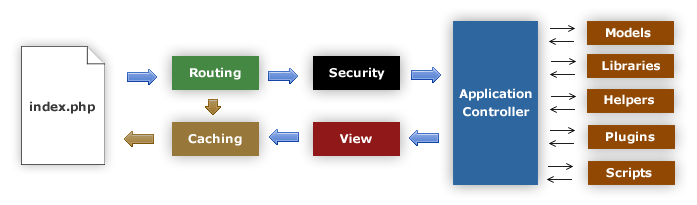
\includegraphics[width=1.0\textwidth]{appflowchart}  
	\caption[\textit{Flow Chart} Aplikasi]{\textit{Flow Chart} Aplikasi} 
	\label{fig:flow} 
\end{figure} 

\begin{enumerate}
	\item File \textit{index.php} berfungsi sebagai \textit{front controller} dan menginisialisasi \textit{resource} utama yang dibutuhkan untuk menjalankan \textit{CodeIgniter}.
	\item \textit{Router} memeriksa \textit{HTTP request} untuk menentukan apa yang harus dilakukan.
	\item Jika terdapat \textit{file cache}, maka akan langsung dikirimkan ke \textit{browser}. \textit{File cache} merupakan data yang pernah diakses oleh pengguna. Data tersebut dapat berupa teks, gambar atau \textit{file}. 
	\item \textit{HTTP request} dan data pengguna yang dikirim akan terlebih dahulu disaring untuk alasan keamanan. \textit{Application controller} akan dimuat setelah proses penyaringan selesai.
	\item \textit{Controller} akan memuat kelas \textit{Model, library} utama dan kelas bantuan.
	\item \textit{View} akan memuat tampilan akhir dan dikirim ke web \textit{browser}. Jika \textit{caching} diaktifkan, maka tampilan dimasukan ke dalam \textit{cache} terlebih dahulu sehingga pada permintaan selanjutnya tampilan tersebut dapat diakses lebih cepat.
\end{enumerate}

\subsection{\textit{Model-View-Controller}}
\label{sec:mvc}
\textit{CodeIgniter} merupakan \textit{framework} yang menggunaakan pola pengembangan \textit{Model-View-Controller}. \textit{MVC} adalah pendekatan perangkat lunak yang memisahkan logika aplikasi dari presentasi. Hal tersebut memungkinkan halaman web pengguna memiliki \textit{scripting} yang sedikit karena presentasi terpisah dari \textit{scripting} PHP~\cite{bcit:17:cidoc}. \\

	\subsubsection{\textit{Model}}
	\textit{Model} merepresentasikan bagian struktur data pengguna. Biasanya kelas \textit{Model} berisi fungsi-fungsi yang membantu pengguna untuk mengambil, menyimpan, dan memperbarui informasi pada \textit{database}. Berikut ini adalah beberapa hal penting yang terdapat pada \textit{Model}:
	\begin{itemize}
		\item Susunan dari \textit{Model} \\
		Kelas \textit{Model} berada di direktori \path{application/models/}. \textit{Model} dapat disimpan ke dalam sub direktori. Bentuk dasar kode pada kelas \textit{model} digambarkan seperti berikut ini:
		\begin{lstlisting}[basicstyle=\ttfamily, frame=single,
columns=fullflexible, keepspaces=true, breaklines=true]
class Model_name extends CI_Model {
	public function_construct()
	{
		parent::_construct();
		//constructor code
	}
}
\end{lstlisting}
		
		\textit{Model\_name} adalah nama kelas dari kelas \textit{model} yang pengguna buat. Penamaan kelas \textit{Model} harus dimulai dengan huruf kapital. Selain itu, kelas \textit{model} harus merupakan turunan (\textit{class CI\_Model} atau \textit{MY\_Model}).
		
		\item Menghubungkan Sebuah \textit{Model} \\
		Pada dasarnya \textit{model} akan dimuat dan dipanggil dari \textit{method} atau fungsi yang ada pada \textit{controller}. Untuk menghubungkan \textit{model}, pengguna harus menggunakan method berikut:
		\begin{lstlisting}[basicstyle=\ttfamily, frame=single,
columns=fullflexible, keepspaces=true, breaklines=true]
$this->load->model('model_name');
\end{lstlisting}
		
		Jika \textit{model} yang pengguna buat terletak di dalam sebuah sub-direktori, maka pengguna harus menyertakan alamat relatif \textit{(relative path)} dari \textit{model} yang dibuat. Sebagai contoh, jika \textit{model} yang pengguna buat berlokasi di \path{application/models/blog/Queries.php} pengguna dapat menghubungkannya dengan cara:
		\begin{lstlisting}[basicstyle=\ttfamily, frame=single,
columns=fullflexible, keepspaces=true, breaklines=true]
$this->load->model('blog/queries');
\end{lstlisting}
		
		Pengguna dapat mengakses \textit{method} yang terdapat pada \textit{model} menggunakan sebuah objek dengan nama yang sama dengan nama kelas yang pengguna buat sebelumnya:
		\begin{lstlisting}[basicstyle=\ttfamily, frame=single,
columns=fullflexible, keepspaces=true, breaklines=true]
$this->load->model('model_name');
		
$this->model_name->method();
\end{lstlisting}
		
		Jika pengguna ingin menggunakan objek yang berbeda untuk sebuah \textit{model}, maka pengguna dapat menggunakan penamaan (alias) di parameter kedua:
		\begin{lstlisting}[basicstyle=\ttfamily, frame=single,
columns=fullflexible, keepspaces=true, breaklines=true]
$this->load->model('model_name', 'foobar');
	
$this->foobar->method();
\end{lstlisting}
		
		Berikut merupakan contoh sebuah \textit{controller} yang terhubung dengan sebuah \textit{model} dan menampilkan data hasil olahan \textit{model} ke \textit{view}:
		\begin{lstlisting}[basicstyle=\ttfamily, frame=single,
columns=fullflexible, keepspaces=true, breaklines=true]
class Blog_controller extends CI_Controller {
			
	public function blog()
	{
		$this->load->model('blog');
		
		$data['query'] = $this->blog->data_sepuluh
		_artikel_terakhir();
		
		$this->load->view('blog', $data);
	}
}
\end{lstlisting}
		
		\item \textit{Auto-loading Model} \\
		\textit{Auto-loading} (menghubungkan secara otomatis) model tertentu secara global dapat pengguna lakukan dengan menggunakan pengaturan yang ada pada berkas \path{application/config/autoload.php}. Kode yang ditambahkan untuk menghubungkan \textit{model} secara otomatis selama sistem berjalan adalah \textit{\$autoload['model'] = array('model\_name');}
		
		\item Koneksi ke \textit{Database} \\
		Ketika sebuah \textit{model} dipanggil, \textit{model} tidak akan terhubung ke \textit{database} secara otomatis. Beberapa opsi yang dapat digunakan untuk menghubungkan \textit{model} ke \textit{database}:
		\begin{itemize}
			\item Pengguna dapat menghubungkan dengan menggunakan metode standar \textit{database} antara \textit{class Controller} atau \textit{class Model}. Metode standar database dibagi menjadi dua cara yaitu \textit{auto connect} dan \textit{manual connect}. Fitur auto connect akan memuat kelas database pada setiap halaman. Manual connect dapat digunakan ketika pengguna menginginkan halaman tertentu yang dapat terhubung dengan database.\\
			\item Pengguna dapat mengatur sebuah \textit{model} melakukan \textit{auto-connect} dengan menambahkan nilai \textit{TRUE} (boolean) di parameter ketiga atau mengatur konektivitas sebagaimana yang telah didefinisikan di dalam \textit{file} \path{application/config/database.php}
			\begin{lstlisting}[basicstyle=\ttfamily, frame=single,
columns=fullflexible, keepspaces=true, breaklines=true]
$this->load->model('model_name', '', TRUE);
\end{lstlisting}
			\item Pengguna dapat mengatur koneksi secara manual dengan menambahkan \textit{item-item} berupa \textit{array} pada \textit{parameter} ketiga seperti contoh berikut:
			\begin{lstlisting}[basicstyle=\ttfamily, frame=single,
columns=fullflexible, keepspaces=true, breaklines=true]
$config['hostname'] = 'localhost';
$config['username'] = 'username';
$config['password'] = 'katasandi';
$config['database'] = 'database_name';
$config['dbdriver'] = 'mysqli';
$config['dbprefix'] = '';
$config['pconnect'] = FALSE;
$config['db_debug'] = TRUE;
			
$this->load->model('model_name', '', $config);
\end{lstlisting}
		\end{itemize}
	\end{itemize}
	
	\subsubsection{\textit{View}}
	\textit{View} merupakan informasi yang akan ditampilkan kepada pengguna. Umumnya \textit{View} merupakan sebuah halaman web, namun pada \textit{CodeIgniter}, \textit{View} dapat berupa bagian-bagian halaman seperti \textit{header} atau \textit{footer}. \textit{View} tidak pernah dipanggil secara langsung, melainkan harus melalui \textit{controller} karena dalam \textit{framework} \textit{MVC}, \textit{controller} berfungsi sebagai pengatur. Untuk memuat tampilan tertentu, pengguna dapat menggunakan \textit{method} berikut:
	\begin{lstlisting}[basicstyle=\ttfamily, frame=single,
columns=fullflexible, keepspaces=true, breaklines=true]
$this->load->view('name');
\end{lstlisting}
	
	\textit{CodeIgniter} dapat menangani beberapa panggilan \textit{method} \textit{\$this->load->view()} dari dalam \textit{controller}. Jika lebih dari satu panggilan terjadi, maka panggilan tersebut ditambahkan bersama. Contohnya pengguna ingin memiliki \textit{header view, menu view, content view} dan \textit{footer view}. Kode program yang digunakan seperti berikut:
	\begin{lstlisting}[basicstyle=\ttfamily, frame=single,
columns=fullflexible, keepspaces=true, breaklines=true]
class Page{
	public function INDEX(){
		$data['page_title'] = 'Your title';
		$load->view('header');
		$load->view('menu');
		$load->view('content', $data);
		$load->view('footer');
	}
}
\end{lstlisting}
	
	\subsubsection{\textit{Controller}}
	\textit{Controller} berfungsi sebagai perantara antara \textit{Model}, \textit{View} dan \textit{resource} lain yang dibutuhkan untuk memproses \textit{HTTP request} dan menghasilkan halaman web. \textit{Controller} merupakan sebuah kelas yang dinamakan demikian agar dapat dikaitkan dengan URI. Sebagai contoh URI \path{example.com/index.php/blog/}. Pada contoh tersebut \textit{segment} terakhir dari URI adalah \textit{blog}, sehingga \textit{CodeIgniter} akan mencari kelas \textit{controller} bernama \textit{Blog.php} dan memuatnya ke dalam \textit{browser}. Nama \textit{controller} harus diawali dengan huruf kapital. Selain itu controller juga harus merupakan turunan kelas "\textit{CI\_Controller}".
	Contoh yang benar :
\begin{lstlisting}[basicstyle=\ttfamily, frame=single,
columns=fullflexible, keepspaces=true, breaklines=true]
<?php
class Blog extends CI_Controller {

}
\end{lstlisting}
	
	Contoh yang salah :
\begin{lstlisting}[basicstyle=\ttfamily, frame=single,
columns=fullflexible, keepspaces=true, breaklines=true]
<?php
class blog extends CI_Controller {

}
\end{lstlisting} 

	Berikut beberapa hal penting yang terdapat pada \textit{Controller}:
	\begin{itemize}
		\item \textit{Method} \\
		Untuk menjalankan suatu \textit{method}, pengguna perlu menuliskannya pada segmen kedua URI. Berikut beberapa \textit{method} yang dibuat pada sebuah \textit{controller}:
\begin{lstlisting}[basicstyle=\ttfamily, frame=single,
columns=fullflexible, keepspaces=true, breaklines=true]
<?php
class Blog extends CI_Controller {
		public function index()
		{
			echo 'Hello World!';
		}
		
		public function comments()
		{
			echo 'Look at this!';
		}
		
		public function shoes($sandals, $id)
		{
			echo $sandals;
			echo $id;
		}
}
\end{lstlisting}
		Jika pengguna memuat URL \path{example.com/index.php/blog/comments}, maka method \textit{comments()} akan dijalankan pada \textit{controller} \textit{Blog.php}. \textit{Method index()} akan dijalankan jika bagian kedua URI kosong. Jika URI mengandung lebih dari dua segment, maka segmen-segmen tersebut akan dimasukan ke dalam \textit{method} sebagai parameter. Contoh: pengguna memuat URL \path{example.com/index.php/blog/shoes/sandals/123}. Segmen "\textit{sandals}" dan "123" akan dimasukan sebagai \textit{parameter} ke dalam \textit{method shoes}.
		
		\item \textit{Default Controller} \\
		\textit{CodeIgniter} dapat diperintahkan untuk menjalankan \textit{default controller} jika tidak terdapat URI. Hal ini umumnya terjadi ketika terdapat permintaan menggunakan URL dasar \textit{website}. Penentuan \textit{default controller} terdapat pada \textit{file} \path{application/config/routes.php}. Berikut contoh penentuan \textit{default controller}:
\begin{lstlisting}[basicstyle=\ttfamily, frame=single,
columns=fullflexible, keepspaces=true, breaklines=true]
$route['default_controller'] = 'blog';
\end{lstlisting} 
		\textit{Blog} merupakan nama kelas \textit{controller} yang ingin digunakan. Jika pengguna mengakses file \textit{index.php} utama tanpa menentukan segmen URI, maka akan dijalankan \textit{controller} \textit{Blog}.
		
%		\item \textit{Processing Output} \\
%		\textit{CodeIgniter} memiliki kelas \textit{output} yang menangani pengiriman data ke \textit{web browser} secara otomatis. Dalam beberapa kasus saat pengguna ingin mengubah cara pengiriman data tersebut, CodeIgnite\textit{}r akan menambahkan \textit{method} bernama "\_output()" ke \textit{controller} terkait. Jika controller memiliki method bernama "\_output()" maka controller tersebut akan selalu dipanggil oleh kelas "\textit{output}".
%		Contoh penggunaan method "\_output()" : 
%\begin{lstlisting}[basicstyle=\ttfamily, frame=single,
%columns=fullflexible, keepspaces=true, breaklines=true]
%public function _output(\$output)
%{
%	echo $output;
%}
%\end{lstlisting}
		
		\item \textit{Private Method}\\
		\textit{Method-method} dengan tipe \textit{private} tidak dapat diakses oleh publik. \textit{Method} ini hanya dapat diakses oleh \textit{method} lain dalam \textit{controller} yang sama dan \textit{method} ini juga tidak dapat diakses melalui URL. Contoh penulisan \textit{private method}:
		\begin{lstlisting}[basicstyle=\ttfamily, frame=single,
columns=fullflexible, keepspaces=true, breaklines=true]
private function _utility()
{
	// kode program
}
\end{lstlisting}
		
		\textit{Method} di atas tidak dapat diakses dengan cara pemanggilan method yang umum seperti berikut:
		\begin{lstlisting}[basicstyle=\ttfamily, frame=single,
columns=fullflexible, keepspaces=true, breaklines=true]
example.com/index.php/blog/_utility/
\end{lstlisting}
		
		\item Mengorganisir \textit{Controller} ke Dalam Sub Direktori \\
		\textit{CodeIgniter} mengizinkan pengguna untuk mengorganisir \textit{controller} ke dalam sub direktori. Pengguna dapat membuat sub direktori di dalam direktori \path{application/controllers/} dan menyimpan kelas \textit{controller} ke direktori tersebut. Ketika menggunakan fitur ini, pengguna harus menspesifikasikan folder tersebut ke dalam URI. Berikut contoh pemanggilan controller yang berada di dalam sub direktori:
		Sebuah \textit{controller} berlokasi pada direktori \path{application/controllers/products/Shoes.php}. Untuk memanggil controller tersebut, URI pengguna yang tampil akan seperti \path{example.com/index.php/products/shoes/show/123}.
	\end{itemize}

%\textit{CodeIgniter} memiliki pendekatan yang cukup fleksibel terhadap \textit{MVC} karena \textit{Model} tidak selalu diperlukan. Para pengguna dapat membangun aplikasi hanya menggunakan \textit{Controller} dan \textit{View}. Hal tersebut dapat dilakukan jika pengguna tidak memerlukan adanya pemisahan tambahan atau pengguna merasa bahwa menggunakan sebuah \textit{Model} membutuhkan kompleksitas yang lebih tinggi~\cite{bcit:17:cidoc}. 

\section{\textit{Sharif Judge}}
\label{sec:sharifjudge} 

\textit{Sharif Judge} adalah \textit{online judge} gratis untuk bahasa pemrograman C, C++, Java dan Python. Perangkat lunak ini diciptakan oleh Mohammad Javad Naderi pada tahun 2014 dan bersifat \textit{open source}. Antarmuka \textit{Sharif Judge} ditulis menggunakan bahasa pemrograman PHP (\textit{framework CodeIgniter}) dan \textit{backend} menggunakan \textit{BASH} \cite{mjnaderi:14:sharifjudge}.
\textit{Sharif Judge} memiliki beberapa fitur seperti:
\begin{itemize}
	\item Terdapat beberapa peran (\textit{role}) \textit{users} yaitu \textit{admin, head instructor, instructor, student}
	\item \textit{Sandboxing} (belum diterapkan untuk \textit{phyton}). \textit{Sandboxing} adalah sebuah mekanisme yang dapat menjalankan aplikasi dalam lingkungan virtual yang aman.
	\item Deteksi kecurangan (mendeteksi kode yang mirip) menggunakan \textit{Moss}
	\item Pengaturan untuk menilai keterlambatan pengiriman
	\item Antrian pengiriman
	\item Mengunduh hasil dalam bentuk \textit{file excel}
	\item Mengunduh kode yang telah dikirim dalam bentuk \textit{file zip}
	\item Metode "\textit{Output Comparison}" dan "\textit{Tester Code}" untuk memeriksa kebenaran dari hasil keluaran.
	\item Menambahkan beberapa pengguna sekaligus
	\item Deskripsi \textit{problem} (\textit{PDF/Markdown/HTML})
	\item Penilaian ulang (\textit{rejudge})
	\item Papan nilai
	\item Notifikasi
\end{itemize}

\subsection{Instalasi}
Untuk menjalankan \textit{Sharif Judge}, dibutuhkan sebuah server \textit{Linux} dengan persyaratan berikut ~\cite{mjnaderi:14:sharifjudgedoc}:
\begin{itemize}
	\item \textit{Webserver} menjalankan PHP versi 5.3 atau yang lebih baru
	\item Pengguna harus dapat menjalankan PHP dari \textit{command line}. Pada \textit{Ubuntu}, pengguna perlu menginstall paket \textit{php5-cli}
	\item \textit{Mysql database} (dengan ekstensi \textit{mysqli} untuk PHP) atau \textit{PostgreSql database}
	\item PHP harus memiliki akses untuk menjalankan \textit{shell commands} menggunakan fungsi \textit{shell\textunderscore exec}. Contohnya seperti \textit{command} di bawah ini: 
		\begin{lstlisting}[basicstyle=\ttfamily, frame=single,
columns=fullflexible, keepspaces=true, breaklines=true]
echo shell_exec("php -v");
\end{lstlisting}
	\item Perkakas yang digunakan untuk melakukan proses kompilasi dan menjalankan kode yang dikumpulkan adalah (\textit{gcc, g++, javac, java, python2, python3 commands})
	\item \textit{Perl} lebih baik diinstall untuk alasan ketepatan waktu, batas memori dan memaksimalkan batas ukuran pada \textit{output} kode yang dikirimkan. \textit{Perl} merupakan salah satu bahasa pemrograman yang dapat digunakan untuk membangun perangkat lunak.
\end{itemize}


Jika persyaratan di atas telah terpenuhi, maka instalasi dapat dilakukan dengan cara sebagai berikut:
\begin{itemize}
	\item Mengunduh versi terakhir dari \textit{Sharif Judge} dan \textit{unpack} hasil download di direktori \textit{public html}
	\item Memindahkan folder \textit{system} dan \textit{application} keluar dari \textit{public directory} dan
	masukan \textit{path} lengkap di \textit{file index.php} 
	\begin{lstlisting}[basicstyle=\ttfamily, frame=single,
columns=fullflexible, keepspaces=true, breaklines=true]
$system_path = '/home/mohammad/secret/system';
$application_folder = '/home/mohammad/secret/application';
\end{lstlisting}
	\item Membuat sebuah \textit{Mysql} atau \textit{PostgreSql} \textit{database} untuk \textit{Sharif Judge}. Jangan menginstall paket koneksi \textit{database} untuk \textit{C/C++, Java}, atau \textit{Python}
	\item Mengatur koneksi \textit{database} di file \path{application/config/database.php}. Pengguna dapat menggunakan awalan untuk nama tabel.
	\begin{lstlisting}[basicstyle=\ttfamily, frame=single,
columns=fullflexible, keepspaces=true, breaklines=true]
/*  Enter database connection settings here:  */
'dbdriver' => 'postgre',    // database driver (mysqli, postgre)
'hostname' => 'localhost',  // database host
'username' => `,           // database username
'password' => `,           // database password
'database' => `,           // database name
'dbprefix' => 'shj_',       // table prefix
/**********************************************/
\end{lstlisting}
	\item Membuat direktori \textit{application/cache/Twig} agar dapat ditulis oleh PHP
	\item Membuka halaman utama \textit{Sharif Judge} pada web \textit{browser} dan ikuti proses instalasi berikutnya
	\item \textit{Log in} menggunakan akun \textit{admin}
	\item Memindahkan folder \textit{tester} dan \textit{assigments} di luar \textit{public directory} lalu simpan \textit{path} lengkap di halaman \textit{Settings}. Dua folder tersebut harus dapat ditulis oleh PHP. \textit{File-file} yang diunggah akan disimpan di folder \textit{assigments} sehingga tidak dapat diakses publik.
\end{itemize}

\subsection{\textit{Clean URLs}}
Secara \textit{default}, \textit{index.php} merupakan bagian dari seluruh \textit{URLs} yang ada pada \textit{Sharif Judge} ~\cite{mjnaderi:14:sharifjudgedoc}. Berikut contoh URLs yang dihasilkan oleh \textit{Sharif Judge}:
\begin{itemize}
	\item \path{http://example.mjnaderi.ir/index.php/dashboard}
	\item \path{http://example.mjnaderi.ir/index.php/users/add}
\end{itemize}

Pengguna dapat menghilangkan \textit{index.php} di atas dan memiliki \textit{URLs} yang baik jika sistem pengguna mendukung \textit{URL rewriting}. \textit{URL rewriting} adalah proses mengubah parameter yang terdapat pada URL. Berikut contoh \textit{URL} yang telah melewati proses \textit{URL rewriting}:
\begin{itemize}
	\item \path{http://example.mjnaderi.ir/dashboard}
	\item \path{http://example.mjnaderi.ir/users/add}
\end{itemize}

Untuk menggunakan \textit{clean urls}, pengguna perlu melakukan beberapa perubahan yaitu:
\begin{itemize}
	\item Mengubah nama \textit{file .htaccess2} menjadi \textit{.htaccess} yang berlokasi di direktori utama \textit{Sharif Judge}. \textit{.htaccess} merupakan sebuah konfigurasi file untuk digunakan pada web server.
	\item Mengubah \textit{\$config['index\_page'] = 'index.php';} menjadi \textit{\$config['index\_page'] = '';} pada file \path{application/config/config.php}.
\end{itemize}

\subsection{\textit{Users}}
Pada \textit{Sharif Judge}, \textit{users} dibagi menjadi 4 \textit{role}. Keempat \textit{role} tersebut adalah \textit{Admins, Head Instructor, Instructor, }dan \textit{Students}
Tabel~\ref{tab:userrole} menunjukan \textit{level users}~\cite{mjnaderi:14:sharifjudgedoc}.

\begin{table}[H] %atau h saja untuk "kira kira di sini"
	\centering 
	\caption{\textit{User Roles Table}}
	\label{tab:userrole}
	\begin{tabular}{|c|c|}
		\hline
		\textit{\textbf{User Role}} & \textit{\textbf{User Level}} \\
		\hline
		\textit{Admin} & 3 \\
		\hline
		\textit{Head Instructor} & 2 \\
		\hline
		\textit{Instructor} & 1 \\
		\hline
		\textit{Student} & 0 \\
		\hline		
	\end{tabular} 
\end{table}

Setiap \textit{users} dapat melakukan aksi yang berbeda-beda. Aksi yang dapat dilakukan para \textit{users} akan disesuaikan dengan \textit{level} masing-masing. Tabel~\ref{tab:useraction} menunjukan aksi-aksi yang dapat dilakukan setiap \textit{users} dengan \textit{level} yang berbeda.
\begin{table}[H] %atau h saja untuk "kira kira di sini"
	\centering 
	\caption{\textit{Permission Table}}
	\label{tab:useraction}
	\begin{tabular}{|l|c|c|c|c|}
		\hline
		Aksi & \textit{Admin} & \textit{Head Instructor} & \textit{Instructor} & \textit{Student} \\
		
		\hline
		Mengubah \textit{Settings} & \ding{51} & \ding{53} & \ding{53} & \ding{53} \\
		Menambah/Menghapus \textit{users} & \ding{51} & \ding{53} & \ding{53} & \ding{53} \\
		Mengubah Peran \textit{users} & \ding{51} & \ding{53} & \ding{53} & \ding{53} \\
		Menambah/Menghapus/Mengubah \textit{Assignment} & \ding{51} & \ding{51} & \ding{53} & \ding{53} \\
		Mengunduh \textit{Test} & \ding{51} & \ding{51} & \ding{53} & \ding{53} \\
		
		Menambah/Menghapus/Mengubah Notifikasi & \ding{51} & \ding{51} & \ding{53} & \ding{53} \\
		\textit{Rejudge} & \ding{51} & \ding{51} & \ding{53} & \ding{53} \\
		Melihat/\textit{Pause}/Melanjutkan/\textit{Submission Queue} & \ding{51} & \ding{51} & \ding{53} & \ding{53} \\
		Mendeteksi Kode yang Mirip & \ding{51} & \ding{51} & \ding{53} & \ding{53} \\
		Melihat Semua Kode & \ding{51} & \ding{51} & \ding{51} & \ding{53} \\
		
		Mengunduh Kode Final& \ding{51} & \ding{51} & \ding{51} & \ding{53} \\
		Memilih \textit{Assignment} & \ding{51} & \ding{51} & \ding{51} & \ding{51} \\
		\textit{Submit} & \ding{51} & \ding{51} & \ding{51} & \ding{51} \\
		
		\hline
		
	\end{tabular} 
\end{table}

Pengguna dapat menambahkan \textit{users} dengan mengklik pada bagian \textit{Add Users} di halaman \textit{Users}. Pengguna harus mengisi semua informasi yang ada pada \textit{text area}. Baris dimulai dengan komentar \textit{\#}. Setiap baris lainnya mewakili pengguna dengan sintaks berikut:
\begin{lstlisting}[basicstyle=\ttfamily, frame=single,
columns=fullflexible, keepspaces=true, breaklines=true]
USERNAME EMAIL PASSWORD ROLE
	
* Usernames dapat berisikan huruf kecil atau nomor dan harus terdiri 
  antara 3 sampai 20 karakter.
* Passwords harus terdiri antara 6 sampai 30 karakter.
* Pengguna dapat menggunakan RANDOM[n] untuk menghasilkan password 
  acak yang terdiri dari n-digit karakter.
* ROLE harus terdiri dari salah satu ini: `admin`, `head_instructor`, 
  `instructor`, `student`
\end{lstlisting}

Berikut contoh penggunaan sintaks untuk menambahkan \textit{users}:
\begin{lstlisting}[basicstyle=\ttfamily, frame=single,
columns=fullflexible, keepspaces=true, breaklines=true]
# This is a comment!
# This is another comment!
instructor instructor@sharifjudge.ir 123456 head_instructor
instructor2 instructor2@sharifjudge.ir random[7] instructor
student1 st1@sharifjudge.ir random[6] student
student2 st2@sharifjudge.ir random[6] student
student3 st3@sharifjudge.ir random[6] student
student4 st4@sharifjudge.ir random[6] student
student5 st5@sharifjudge.ir random[6] student
student6 st6@sharifjudge.ir random[6] student
student7 st7@sharifjudge.ir random[6] student
\end{lstlisting}

\subsection{Menambah \textit{Assignment}}
Pengguna dapat menambahkan \textit{assignment} dengan cara mengklik \textit{Add} di halaman \textit{assigments}~\cite{mjnaderi:14:sharifjudgedoc}. Pengguna akan melihat halaman seperti Gambar~\ref{fig:addass}.
\begin{figure}[H]
	\centering  
	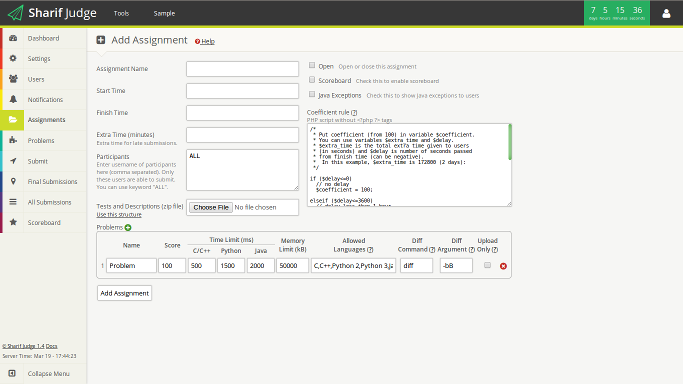
\includegraphics[width=1.0\textwidth]{add_assignment}  
	\caption[Tampilan Halaman \textit{Assignments}]{Tampilan Halaman \textit{Assignments}} 
	\label{fig:addass} 
\end{figure} 

Berikut ini adalah pengaturan yang terdapat pada halaman \textit{Add Assignments}:
\begin{itemize}
	\item \textit{Assignment Name} \\
	Nama \textit{assignment} yang akan ditampilkan dalam daftar \textit{assignment}.
	
	\item \textit{Start Time} \\
	Peserta tidak dapat mengumpulkan \textit{assignment} sebelum \textit{"Start Time"}. Format yang digunakan untuk pengaturan \textit{start time} adalah \textit{MM/DD/YYYY HH:MM:SS}. Contoh: \textit{08/31/2013 12:00:00}
	
	\item \textit{Finish Time, Extra Time}\\
	Peserta tidak dapat mengumpulkan \textit{assignment} setelah \textit{Finish Time + Extra Time}. \textit{Assignment} yang telat akan dikalikan dengan koefisien tertentu. Pengguna harus menulis \textit{script} PHP untuk menghitung koefisien pada bidang \textit{"Coefficient Rule"}. Format yang digunakan untuk pengaturan \textit{finish time} adalah \textit{MM/DD/YYYY HH:MM:SS}. Contoh: \textit{08/31/2013 23:59:59}. "\textit{Extra Time}" akan terhitung dalam satuan menit. Pengguna juga dapat menggunakan operator aritmatika seperti *, -, +, /. Contoh \textit{120} (2 jam) atau \textit{48*60} (2 hari).
	
	\item \textit{Participants} \\
	Pengaturan ini berfungsi untuk membatasi peserta yang dapat mengumpulkan \textit{assignment}. Pengguna dapat menggunakan kata kunci \textit{ALL} pada kolom \textit{Participants} untuk mengijinkan seluruh peserta agar dapat mengumpulkan \textit{assignment}. Untuk membatasi peserta tertentu, pengguna dapat memasukan \textit{username} peserta pada kolom \textit{Participants}. Setiap \textit{username} dapat dipisahkan menggunakan tanda koma. Contoh: \textit{admin, instructor1, instructor2, student1, student2, student3, student4}.
	
	\item \textit{Open} \\
	Pengguna dapat membuka atau menutup \textit{assignment} menggunakan pilihan ini. Jika pengguna menutup \textit{assignment}, \textit{non-student users} masih dapat mengumpulkan \textit{assignment}.
	
	\item Scoreboard \\
	Pengguna dapat mengaktifkan atau mematikan papan nilai dengan menggunakan pilihan ini.
	
	\item \textit{Java Exceptions}\\
	Pengguna dapat mengaktifkan dan mematikan \textit{java exceptions} yang ditunjukan kepada \textit{students}. Perubahan pada pilihan ini tidak berdampak pada kode yang sebelumnya sudah dinilai. Nama \textit{exception} akan muncul jika pada \textit{file} path{tester/java\_exceptions\_list} berisikan nama \textit{exception} tersebut. Berikut hasil \textit{exception} yang ditunjukan jika pengguna mengaktifkan pengaturan \textit{Java Exceptions}: 
	\begin{lstlisting}[basicstyle=\ttfamily, frame=single,
columns=fullflexible, keepspaces=true, breaklines=true]
Test 1
ACCEPT
Test 2
Runtime Error (java.lang.ArrayIndexOutOfBoundsException)
Test 3
Runtime Error (java.lang.ArrayIndexOutOfBoundsException)
Test 4
ACCEPT
Test 5
ACCEPT
Test 6
ACCEPT
Test 7
ACCEPT
Test 8
Runtime Error (java.lang.ArrayIndexOutOfBoundsException)
Test 9
Runtime Error (java.lang.StackOverflowError)
Test 10
Runtime Error (java.lang.ArrayIndexOutOfBoundsException)
\end{lstlisting}
	
	\item \textit{\textit{Coefficient Rule}} \\
	Pengguna dapat menulis \textit{script} PHP pada bagian ini. Pengguna harus memasukan koefisien (dari 100) pada variabel \textit{\$coefficient}. Pengguna dapat menggunakan variabel \textit{\$extra\_time} dan \textit{\$delay}. \textit{\$extra\_time} merupakan total waktu ekstra yang diberikan kepada \textit{users} dalam satuan detik dan \textit{\$delay} merupakan jumlah detik berlalu dari waktu selesai (bisa negatif). \textit{Script} PHP pada bagian ini tidak mengandung \textit{tags <?php , <? , ?>}. Berikut contoh \textit{\$extra\_time} 172800 (2 hari):
	\begin{lstlisting}[basicstyle=\ttfamily, frame=single,
columns=fullflexible, keepspaces=true, breaklines=true]
if ($delay<=0)
// no delay
$coefficient = 100;

elseif ($delay<=3600)
// delay less than 1 hour
$coefficient = ceil(100-((30*$delay)/3600));

elseif ($delay<=86400)
// delay more than 1 hour and less than 1 day
$coefficient = 70;

elseif (($delay-86400)<=3600)
// delay less than 1 hour in second day
$coefficient = ceil(70-((20*($delay-86400))/3600));

elseif (($delay-86400)<=86400)
// delay more than 1 hour in second day
$coefficient = 50;

elseif ($delay > $extra_time)
// too late
$coefficient = 0;
\end{lstlisting}
	
	\item \textit{Time Limit} \\
	Pengguna dapat mengatur batas waktu untuk menjalankan kode dalam satuan milisekon. Program yang ditulis menggunakan \textit{Python} dan \textit{Java} biasanya lebih lambat dari \textit{C/C++}.	Oleh karena itu \textit{Python} dan \textit{Java} membutuhkan waktu yang lebih.
	
	\item \textit{Memory Limit} \\
	Pengguna dapat mengatur batas memori dalam satuan \textit{kilobyte}, namun penggunaan \textit{Memory Limit} tidak terlalu akurat.
	
	\item \textit{Allowed Languages} \\
	Pengguna dapat mengatur bahasa untuk setiap \textit{problem} (dipisahkan menggunakan koma). Bahasa yang tersedia seperti \textit{C, C++, Java, Python 2, Python 3, zip, PDF}. Pengguna dapat menggunakan \textit{zip} atau \textit{PDF} jika mengaktifkan pilihan \textit{Upload Only}. Contoh: \textit{C, C++ , zip} atau \textit{Python 2,Python 3} atau \textit{Java ,C}.
	
	\item \textit{Diff Command} \\
	\textit{Command} ini digunakan untuk membandingkan keluaran dengan keluaran yang benar. Secara \textit{default Sharif Judge} menggunakan \textit{diff}, namun pengguna dapat mengubah \textit{command} pada bagian ini.
	
	\item \textit{Diff Arguments} \\
	Pengguna dapat mengatur argumen dari \textit{Diff Command} disini. Untuk melihat daftar lengkap \textit{diff} argumen, pengguna dapat melihat \textit{man diff}. \textit{Sharif Judge} menambahkan dua pilihan baru yaitu \textit{ignore} dan \textit{identical}. \textit{Ignore} akan menghiraukan semua baris baru dan spasi. \textit{Identical} tidak akan menghiraukan apapun namun keluaran dari file yang dikumpulkan harus identik dengan keluaran \textit{test case} agar dapat diterima.
	
	\item \textit{Upload Only} \\
	Jika pengguna mengatur \textit{problem} sebagai \textit{Upload-Only}, maka \textit{Sharif Judge} tidak akan menilai \textit{assignment} pada \textit{problem} tersebut. Pengguna dapat menggunakan \textit{zip} dan \textit{PDF} pada \textit{allowed languages} jika mengaktifkan pilihan ini.
\end{itemize}

\subsubsection{Contoh \textit{Assignment}}

Berikut contoh \textit{assignment} untuk mencoba \textit{Sharif Judge}. Menambah \textit{assignment} dengan mengklik \textit{Add} di halaman \textit{Assignment}. \textit{Assignment} dibagi menjadi 3 \textit{problem}:
\begin{enumerate}
	\item \textit{Problem} 1 (Penjumlahan) \\
	Program pengguna akan menerima masukan bilangan \textit{integer} n, kemudian menerima masukan lagi sebanyak n buah bilangan \textit{integer} dan menampilkan hasil penjumlahan dari n nomor tersebut. Tabel~\ref{tab:tablesum} menunjukan contoh \textit{input} dan \textit{output} untuk \textit{Problem 1}.
	
	\begin{table}[H] %atau h saja untuk "kira kira di sini"
		\centering 
		\caption{\textit{Problem} 1 (Penjumlahan)}
		\label{tab:tablesum}
		\begin{tabular}{|c|c|}
			\hline
			Sample Input & Sample Output\\
			
			\hline
			\multicolumn{1}{|l|}{5} & \multirow{2}{*}{145}\\
			\multicolumn{1}{|l|}{54 78 0 4 9} & \\
			
			\hline
			
		\end{tabular} 
	\end{table}
	
	\item \textit{Problem} 2 (\textit{Max}) \\
	Program pengguna akan menerima masukan bilangan \textit{integer} n, kemudian menerima masukan lagi sebanyak n buah bilangan \textit{integer} dan menampilkan hasil penjumlahan dari dua nilai tertinggi. Tabel~\ref{tab:tablemax} menunjukan contoh \textit{input} dan \textit{output} untuk \textit{Problem 2}.
	
	\begin{table}[H] %atau h saja untuk "kira kira di sini"
		\centering 
		\caption{\textit{Problem} 2 (\textit{Max})}
		\label{tab:tablemax}
		\begin{tabular}{|c|c|}
			\hline
			Sample Input & Sample Output\\
			
			\hline
			\multicolumn{1}{|l|}{7} & \multirow{2}{*}{356}\\
			\multicolumn{1}{|l|}{162 173 159 164 181 158 175} & \\
			
			\hline
			
		\end{tabular} 
	\end{table}
	
	\item \textit{Problem} 2 (\textit{Upload!}) \\
	Pengguna diharuskan mengunggah sebuah \textit{file} \textit{C} atau \textit{zip}. \textit{Problem} ini menggunakan pilihan \textit{"Upload Only} sehingga tidak akan dinilai oleh \textit{Sharif Judge}.
\end{enumerate}

Pengguna dapat menemukan \textit{file zip} pada \textit{folder Assignments}. Berikut susunan pohon dari tugas tiga \textit{problem} di atas:
\begin{lstlisting}[basicstyle=\ttfamily, frame=single,
columns=fullflexible, keepspaces=true, breaklines=true]
.
|-- p1
|   |-- in
|   |   |-- input1.txt
|   |   |-- input2.txt
|   |   |-- input3.txt
|   |   |-- input4.txt
|   |   |-- input5.txt
|   |   |-- input6.txt
|   |   |-- input7.txt
|   |   |-- input8.txt
|   |   |-- input9.txt
|   |   --- input10.txt
|   |-- out
|   |   --- output1.txt
|   |-- tester.cpp
|   --- desc.md
|-- p2
|   |-- in
|   |   |-- input1.txt
|   |   |-- input2.txt
|   |   |-- input3.txt
|   |   |-- input4.txt
|   |   |-- input5.txt
|   |   |-- input6.txt
|   |   |-- input7.txt
|   |   |-- input8.txt
|   |   |-- input9.txt
|   |   --- input10.txt
|   |-- out
|   |   |-- output1.txt
|   |   |-- output2.txt
|   |   |-- output3.txt
|   |   |-- output4.txt
|   |   |-- output5.txt
|   |   |-- output6.txt
|   |   |-- output7.txt
|   |   |-- output8.txt
|   |   |-- output9.txt
|   |   --- output10.txt
|   |-- desc.md
|   --- Problem2.pdf
|-- p3
|   --- desc.md
--- SampleAssignment.pdf
\end{lstlisting}
\textit{Problem} 1 menggunakan metode \textit{"Tester"} untuk mengecek keluaran, sehingga memiliki \textit{file tester.cpp (Tester Script)}. \textit{Problem} 2 menggunakan metode \textit{Output Comparison} untuk mengecek keluaran, sehingga memiliki dua \textit{folder} (\textit{in} dan \textit{out}) yang berisikan \textit{test case}. \textit{Problem} 3 merupakan \textit{problem} yang menggunakan pilihan \textit{Upload-Only}.

\subsubsection{Aturan-aturan \textit{Submission}}
Untuk dapat mengumpulkan jawaban pada sebuah \textit{assignment}, terdapat beberapa aturan yaitu:
\begin{enumerate}
	\item Jawaban tidak dapat dikumpulkan jika waktu sekarang belum melewati \textit{'Start time'} pada \textit{assignment} yang dipilih.
	\item Jawaban tidak dapat dikumpulkan jika waktu sekarang telah melewati \textit{'Finish time'} pada \textit{assignment} yang dipilih.
	\item Jawaban tidak dapat dikumpulkan jika assignment yang dipilih berstatus \textit{close}.
	\item Jawaban tidak dapat dikumpulkan jika peserta tidak terdaftar pada assignment yang dipilih.
\end{enumerate}

Jika seluruh aturan tersebut telah terpenuhi, maka peserta dapat mengumpulkan jawaban masing-masing. Berikut langkah-langkah untuk mengumpulkan jawaban pada sebuah assignment:
\begin{enumerate}
	\item Memilih \textit{assignment} yang ingin dikumpulkan pada halaman \textit{Assignment}.
	\item Pada halaman \textit{Submit}, para peserta dapat memilih \textit{problem} yang ingin dikumpulkan, bahasa pemrograman yang digunakan dan \textit{file} jawaban.
	\item Menekan tombol \textit{Submit} untuk mengumpulkan jawaban.
\end{enumerate}

Setelah menekan tombol \textit{Submit}, pengguna akan diarahkan ke halaman \textit{All Submission}. Pada tahap ini, jawaban para peserta telah berhasil dikumpulkan ke \textit{Sharif Judge}.

\subsection{Struktur Pengujian}

Pengguna harus menyediakan sebuah \textit{file zip} yang berisikan \textit{test cases} ketika menambahkan \textit{assignment}. \textit{File zip} ini dapat berisi folder-folder untuk setiap \textit{problem}. Pengguna harus memberikan nama pada folder sesuai aturan seperti \textit{p1, p2, p3, dst}. \textit{Assignment} yang menggunakan pilihan \textit{Upload-Only} tidak membutuhkan \textit{folder}~\cite{mjnaderi:14:sharifjudgedoc}.

\subsubsection{Metode Pengecekan}
\textit{Sharif Judge} memiliki dua metode pengecekan untuk setiap \textit{problem} yaitu metode \textit{"Input/Output" Comparison} dan metode \textit{Tester}.
\begin{itemize}
	\item \textit{Metode Input/Output Comparison} \\
	Dengan metode ini, pengguna harus memasukan beberapa \textit{file input dan output} pada \textit{folder} \textit{problem}. \textit{Sharif Judge} akan memasukan nilai dari \textit{file input} ke kode \textit{users} dan membandingkan hasil keluaran dari kode \textit{users} dengan \textit{file output}. \textit{Input files} harus berada dalam folder \textit{"in"} dengan nama \textit{input1.text, input2.txt, dst}.\textit{Output files} harus berada dalam folder \textit{"out"} dengan nama \textit{output1.txt, output2.txt, dst}.
	
	\item \textit{Metode Tester} \\
	Dengan metode ini, pengguna harus menyediakan beberapa \textit{file input} dan sebuah \textit{file C++ (tester.cpp)} dan beberapa \textit{file output}. \textit{Sharif Judge} akan memasukan nilai dari \textit{file input} ke kode \textit{users} dan mengambil keluaran dari kode \textit{users}. \textit{tester.cpp} akan mengambil nilai dari \textit{file input, file output, }dan keluaran \textit{users}. Jika keluaran dari kode \textit{users} benar akan mengembalikan nilai 0, sebaliknya jika salah akan mengeluarkan nilai 1. Listing \ref{ls:7} menunjukan contoh kode untuk menulis \textit{tester.cpp}:
	\begin{lstlisting}[basicstyle=\ttfamily, caption=Contoh kode \textit{tester.cpp}, label=ls:7, frame=single,
columns=fullflexible, keepspaces=true, breaklines=true]
/*
* tester.cpp
*/

#include <iostream>
#include <fstream>
#include <string>
using namespace std;
int main(int argc, char const *argv[])
{
	
	ifstream test_in(argv[1]);  /* Stream ini membaca 
	isi file input */
	ifstream test_out(argv[2]); /* Stream ini membaca 
	isi file output */
	ifstream user_out(argv[3]); /* Stream ini membaca 
	isi keluaran users */
	
	/* Kode Pengguna */
	/* Jika keluaran kode user benar, mengembalikan nilai 0, 
	sebaliknya mengembalikan 1 */
	
	...

}
\end{lstlisting}
\end{itemize}

\subsubsection{Contoh \textit{File}}

Pengguna dapat menemukan contoh \textit{file} penguji pada \textit{folder Assignments}. Berikut susunan pohon dari \textit{file} tersebut:
\begin{lstlisting}[basicstyle=\ttfamily, frame=single,
columns=fullflexible, keepspaces=true, breaklines=true]
.
|-- p1
|   |-- in
|   |   |-- input1.txt
|   |   |-- input2.txt
|   |   |-- input3.txt
|   |   |-- input4.txt
|   |   |-- input5.txt
|   |   |-- input6.txt
|   |   |-- input7.txt
|   |   |-- input8.txt
|   |   |-- input9.txt
|   |   --- input10.txt
|   |-- out
|   |   --- output1.txt
|   --- tester.cpp
--- p2
	|-- in
	|   |-- input1.txt
	|   |-- input2.txt
	|   |-- input3.txt
	|   |-- input4.txt
	|   |-- input5.txt
	|   |-- input6.txt
	|   |-- input7.txt
	|   |-- input8.txt
	|   |-- input9.txt
	|   --- input10.txt
	--- out
	|-- output1.txt
	|-- output2.txt
	|-- output3.txt
	|-- output4.txt
	|-- output5.txt
	|-- output6.txt
	|-- output7.txt
	|-- output8.txt
	|-- output9.txt
	--- output10.txt
\end{lstlisting}

\textit{Problem} 1 menggunakan metode \textit{"Tester"} untuk mengecek hasil keluaran, sehingga memiliki \textit{file tester.cpp}. Listing \ref{ls:8} menunjukan isi dari \textit{file tester.cpp} untuk \textit{problem} 1:
\begin{lstlisting}[basicstyle=\ttfamily, caption=Isi \textit{File tester.cpp} Problem 1, label=ls:8, frame=single,
columns=fullflexible, keepspaces=true, breaklines=true]
/*
* tester.cpp
*/

#include <iostream>
#include <fstream>
#include <string>
using namespace std;
int main(int argc, char const *argv[])
{
	
	ifstream test_in(argv[1]);  /* Stream ini membaca 
	isi file input */
	ifstream test_out(argv[2]); /* Stream ini membaca 
	isi file output */
	ifstream user_out(argv[3]); /* Stream ini membaca 
	isi keluaran users */
	
	/* Kode Pengguna */
	/* Jika keluaran kode user benar, mengembalikan nilai 0, 
	sebaliknya mengembalikan 1 */
	/* e.g.: Permasalahan: membaca n nomor dan keluarkan 
	hasil penjumlahannya: */
	
	int sum, user_output;
	user_out >> user_output;
	
	if ( test_out.good() ) // if test's output file exists
	{
		test_out >> sum;
	}
	else
	{
		int n, a;
		sum=0;
		test_in >> n;
		for (int i=0 ; i<n ; i++){
			test_in >> a;
			sum += a;
		}
	}
	
	if (sum == user_output)
		return 0;
	else
		return 1;

}
\end{lstlisting}


\textit{Problem} 2 menggunakan metode \textit{"Input/Output Comparison"} untuk mengecek hasil keluaran, sehingga memiliki dua folder \textit{in} dan \textit{out} yang berisikan \textit{test cases}. \textit{Problem} 3 menggunakan pilihan \textit{Upload-Only}, sehingga tidak memiliki folder apapun.

\subsection{Deteksi Kecurangan}
\textit{Sharif Judge} menggunakan \textit{Moss} untuk mendeteksi kode yang mirip. \textit{Moss (Measure Of Software Similarity)} merupakan sistem otomatis untuk menentukan kemiripan program. Pada saat ini, aplikasi utama \textit{Moss} telah digunakan untuk mendeteksi plagiarisme pada kelas \textit{programming}. Pengguna dapat mengirimkan kode final (yang dipilih oleh \textit{students} sebagai \textit{Final Submission}) ke \textit{server Moss} dengan satu klik~\cite{mjnaderi:14:sharifjudgedoc}.\\

Sebelum menggunakan \textit{Moss} ada beberapa hal yang harus diperhatikan yaitu:
\begin{itemize}
	\item Pengguna harus mendapatkan \textit{Moss user id} dan mengaturnya di \textit{Sharif Judge}. Untuk mendapatkan \textit{Moss user id}, pengguna harus terlebih dahulu mendaftar pada halaman \path{http://theory.stanford.edu/~aiken/moss/}. Pengguna akan mendapatkan sebuah \textit{email} yang berisikan \textit{script perl}. \textit{Moss user id} berada pada \textit{script} tersebut. \\
	Listing \ref{ls:9} menunjukan potongan \textit{perl script} yang berisikan \textit{user id}:

\begin{lstlisting}[basicstyle=\ttfamily, caption=Potongan \textit{perl script}, label=ls:9, frame=single,
columns=fullflexible, keepspaces=true, breaklines=true]
...

$server = 'moss.stanford.edu';
$port = '7690';
$noreq = "Request not sent.";
$usage = "usage: moss [-x] [-l language] [-d] 
		  [-b basefile1] ... [-b basefilen] [-m #] 
		  [-c \"string\"] file1 file2 file3 ...";

#
# The userid is used to authenticate your queries to the server; 
  don't change it!
#
$userid=YOUR_MOSS_USER_ID;

#
# Process the command line options.  This is done in a non-standard
# way to allow multiple -b's.
#
$opt_l = "c";   # default language is c
$opt_m = 10;
$opt_d = 0;

...
}

\end{lstlisting}

 \textit{User id} yang terdapat pada potongan \textit{perl script} di atas, dapat digunakan pada \textit{Sharif Judge} untuk mendeteksi kecurangan. Pengguna dapat menyimpan \textit{user id} di \textit{Sharif Judge} pada halaman \textit{Moss}. \textit{Sharif Judge} akan menggunakan \textit{user id} tersebut di \textit{Moss perl script}.

 \textit{Perl} harus terinstal pada server agar dapat menggunakan \textit{Moss}.

\item Pengguna dianjurkan untuk mendeteksi kode yang mirip setelah waktu \textit{assignment} berakhir, karena para peserta masih dapat mengubah \textit{Final Submissions} masing-masing sebelum waktu habis. Dengan cara tersebut, \textit{Sharif Judge} dapat mengirimkan \textit{Final submissions} para peserta ke \textit{server Moss}.
\end{itemize}

\subsection{\textit{Database}}
Sebuah \textit{database} dibutuhkan untuk menjalankan \textit{Sharif Judge}. \textit{Database} yang dapat digunakan yaitu \textit{Mysql} dan \textit{PostgreSql}. Pada \textit{database} tersebut terdapat beberapa tabel yang secara otomatis dibuat saat proses instalasi \textit{Sharif Judge}. Beberapa tabel tersebut yaitu:
\begin{itemize}
	\item \textit{shj\_assignments} \\
	Tabel ini menyimpan seluruh informasi \textit{assignment} yang ada pada \textit{Sharif Judge}. Atribut yang terdapat pada tabel ini antara lain \textit{id, name, problems, total\_submits, open, scoreboard, javaexceptions, description, start\_time, finish\_time, extra\_time, late\_rule, participants} dan \textit{moss\_update}.
	\item \textit{shj\_notifications} \\
	Tabel ini menyimpan seluruh informasi notifikasi yang ada pada \textit{Sharif Judge}. Atribut yang terdapat pada tabel ini antara lain \textit{id, title, text} dan \textit{time}.
	\item \textit{shj\_problems} \\
	Tabel ini menyimpan seluruh informasi \textit{problem} yang ada pada setiap \textit{assignment}. Atribut yang terdapat pada tabel ini antara lain \textit{assignment, id, name, score, is\_upload\_only, c\_time\_limit, python\_time\_limit, java\_time\_limit, memory\_limit, allowed\_languages, diff\_cmd} dan \textit{diff\_arg}. 
	\item \textit{shj\_queue} \\
	Tabel ini menyimpan seluruh informasi antrian pada saat proses penilaian berlangsung. Atribut yang terdapat pada tabel ini antara lain \textit{id, submit\_id, username, assignment, problem} dan \textit{type}.
	\item \textit{shj\_scoreboard} \\
	Tabel ini menyimpan seluruh informasi \textit{scoreboard} pada setiap \textit{assignment}. Atribut yang terdapat pada tabel ini antara lain \textit{assignment} dan \textit{scoreboard}.
	\item \textit{shj\_session} \\
	Tabel ini menyimpan seluruh informasi \textit{session} setiap peserta \textit{Sharif Judge}. Atribut yang terdapat pada tabel ini antara lain \textit{session\_id, ip\_address, user\_agent, last\_activity} dan \textit{user\_data}.
	\item \textit{shj\_settings} \\
	Tabel ini menyimpan seluruh informasi pengaturan yang ada pada \textit{Sharif Judge}. Atribut yang terdapat pada tabel ini antara lain \textit{shj\_key} dan \textit{shj\_value}.
	\item \textit{shj\_submissions} \\
	Tabel ini menyimpan seluruh informasi jawaban yang telah dikumpulkan ke \textit{Sharif Judge}. Atribut yang terdapat pada tabel ini antara lain \textit{submit\_id, username, assignment, problem, is\_final, time, status, pre\_score, coefficient, file\_name, main\_file\_name} dan \textit{file\_type}.
	\item \textit{shj\_users} \\
	Tabel ini menyimpan seluruh informasi peserta yang terdaftar pada \textit{Sharif Judge}. Atribut yang terdapat pada tabel ini antara lain \textit{id, username, password, display\_name, email, role, passchange\_key, passchange\_time, first\_login\_time, last\_login\_time, selected\_assignment} dan \textit{dasboard\_widget\_positions}.
\end{itemize}

\section{\textit{Twig}}
Pada perangkat lunak \textit{\textit{Sharif Judge}}, kelas view menggunakan \textit{framework} aplikasi yaitu \textit{Twig}. \textit{Twig} merupakan sebuah \textit{template engine modern} untuk \textit{PHP} ~\cite{fabien:09:twig}. Sebuah \textit{template Twig} dapat mengandung \textit{variables} atau \textit{expression} dan \textit{tags}. \textit{Variables} atau \textit{expression} akan diubah pada saat \textit{template Twig} dievaluasi dan \textit{tags} yang akan mengontrol logika dari \textit{template} tersebut. Listing \ref{twig:1} menunjukan template kode yang menunjukan beberapa hal mendasar.

\begin{lstlisting}[language=diff, caption=Template Kode , label=twig:1, basicstyle=\ttfamily, frame=single,
columns=fullflexible, keepspaces=true]
<!DOCTYPE html>
<html>
	<head>
	<title>My Webpage</title>
		</head>
	<body>
		<ul id="navigation">
		
			<li><a href="{{ item.href }}">{{ item.caption }}</a></li>
		
		</ul>
		
		<h1>My Webpage</h1>
		{{ a_variable }}
	</body>
</html>
\end{lstlisting}

Ada dua jenis \textit{delimiters} pada kode di atas, yaitu \{\% ... \%\} dan \{\{ ... \}\}. \textit{Delimiters} \{\% ... \%\} digunakan untuk mengeksekusi sebuah \textit{statements}. Pada kode di atas, \textit{delimiters} \{\% \textit{for item in navigation} \%\} akan mengeksekusi \textit{statements for-loops} atau pengulangan. \textit{Delimiters} \{\{ ... \}\} digunakan untuk menampilkan nilai. Pada kode di atas, \textit{delimiters} \{\{ \textit{item.href} \}\} akan menampilkan nilai \textit{item.href}, \textit{delimiters} \{\{ \textit{item.caption} \}\} akan menampilkan nilai \textit{item.caption} dan \textit{delimiters} \{\{ \textit{a\_variable} \}\} akan menampilkan nilai \textit{a\_variable}.